\section{データ型}
\markright{\arabic{section}. データ型}
他のLispと同様に、型の決まったデータオブジェクトは変数ではない。
どの変数もその値として、どんなオブジェクトも持つことができる。
変数にオブジェクトの型を宣言することが可能であるが、
一般的にコンパイラで高速なコードを生成するための情報としてのみ
使用される。
数値は、ポインタの中で直接値として表現され、
そのほかは、ポインタにより参照されるオブジェクトにより表現される。
Sun4で実行する場合、ポインタおよび数値は図\ref{Pointer}で描かれているように
long wordで表現される。
ポインタのLSBの2ビットは、ポインタ・integer・floatを識別するための
tagビットとして使用されている。
ポインタはtagビットが全てゼロであり、オブジェクトのアドレスとして32ビット全て
使用できるので、EusLispは4GB以上のアドレス空間を利用することができる。

\begin{figure}[hb]
\begin{center}
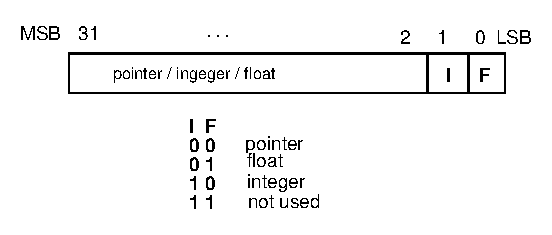
\includegraphics{fig/pointer.ps}
%\epsfile{file=fig/pointer.ps}
\end{center}
\caption{\label{Pointer}ポインタと直接値}
\end{figure}

\subsection{数値}
数値には、integerとfloat(浮動小数点)の2種類があり、
両方とも29ビットの値と1ビットの符号で表現される。
したがって、integerは$-$536,870,912から536,870,911までの範囲となる。
floatは、正および負で4.8E$-$38から3.8E38までの範囲を表現でき、
その有効数字は、十進数で約6桁すなわち浮動小数点誤差は1/1,000,000程度である。

数値は、いつもオブジェクトでなくポインタで表現される。
これは、EusLispのオブジェクト指向の唯一の例外事項である。
しかしながら、数値は決してヒープメモリを無駄にすることがないため、
数値を扱うアプリケーションでは、ガーベージコレクション
の原因とならず有効に動作する。

EusLispは、文字型を持たないため、文字列はintegerで表現される。
文字コード表と無関係なプログラムを書くためには、
%\#$\backslash$
\verb+#\+ 読みだしマクロが役に立つ。しかし、文字が読まれるとき、
数値表現に変換されるため、プリンタは
%\#$\backslash$
\verb+#\+ の表記法に対してどのように再変換すればよいのか解らない。

数値は、図\ref{Pointer}のlong wordの中に2つのtagビットを持っている。
それで、数値計算に使用するときは、シフトまたはマスクすることにより
このビットを消す必要がある。
integerは数値シフトによりMSBの2ビットを無視し、floatはマスクにより
LSBの2ビットを無視する。
VAXのようなアーキテクチャのためにByte swapも必要である。なぜなら、
意味を持つ最小の大きさのByteとして右端の1Byteが使用できないためである。


\subsection{オブジェクト}
数値でない全てのデータは、ヒープにおかれるオブジェクトで表現される。
それぞれのオブジェクトのメモリセルは、オブジェクトヘッダーと
オブジェクト変数のための固定数のスロットを持っている。
ベクトルは、任意の要素から構成されるため、
sizeスロットをヘッダーのすぐ後に持っている。
図\ref{ObjectFig}はオブジェクトとベクトルおよび
オブジェクトのヘッダーを描いたものである。
ここに示す{\em slot}と{\em element}のワードだけがユーザーから
アクセスすることができる。


\begin{figure}[hbt]
\begin{center}
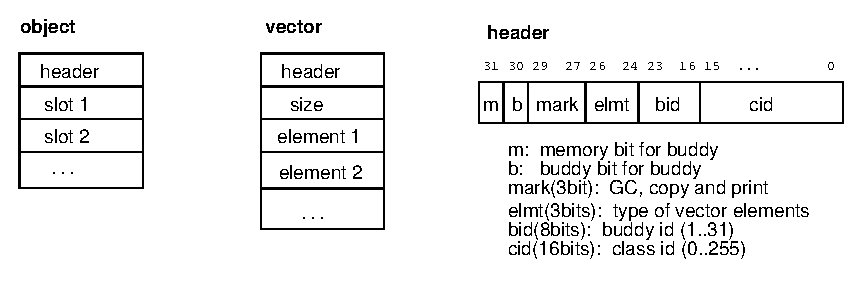
\includegraphics{fig/object.ps}
%\epsfile{file=fig/object.ps}
\end{center}
\caption{\label{ObjectFig}オブジェクト・ベクトル・オブジェクトヘッダーの構造}
\end{figure}

ヘッダーは、6つの部分で構成されている。
MSBの2ビット{\em m}と{\em b}は、フィボナッチバディメモリ管理手法の中で、
隣接セルの終端を示すために使用される。

{\em mark}部分には、3つのマークビットがあり、それぞれ
ガーベージコレクタ用のアクセス可能セルの認識、
プリンタ用の環状オブジェクトの認識(
{\tt \#n=}や{\tt \#n\#}表記法でプリントアウトさせた時)、
{\bf copy-object}用の分割オブジェクトのコピーとして使用される。
{\em elmt}部分は、ベクトル要素として使用可能な7つのデータ型(
{\tt pointer, bit, character, byte, integer, float, foreign-string})
のうち1つを識別するために使用される。
しかしながら、{\em elmt}はクラスの中で利用可能なため、
クラスの構造と無関係なメモリ管理ができ、
要素の高速なアクセスができる。
{\em bid}部分は、メモリセルの物理的大きさを表現する。
31の違った大きさ(16MB以上)のメモリセルをこの5ビットで表現する。
%with relatively finer resolution than the binary buddy method.
下位のshort word (16ビット)は、クラスID(cid)として使用される。
これは、システムのクラステーブルを経由してオブジェクトのクラスを
引き出すために使用される。
このクラスIDは、伝統的なLispの型tagとみなすことができる。
cidは下位8ビットのみが使用され、上位8ビットは無視される。
したがって、クラスの最大数は256が限界であるけれども、
システムのクラステーブルにもっとメモリを配置するように
EusLispを再構築することによって65536まで限界を引き上げることができる。

\subsection{クラス継承}

オブジェクトのデータ構造はクラスによって定義され、そして、それらの動作は
クラス内のメソッドに定義されている。
EusLispにおいて、数ダースのクラスが図\ref{ClassHierarchy}に書かれているように
木構造化された継承のなかにすでに定義されている。
{\bf class-hierarchy}関数を用いれば、実際の継承構造を見ることができる。
左端のクラスobjectは、EusLisp内の全てのクラスの根幹となるスーパークラスである。
ユーザーが定義したクラスは、これらの内部クラスのどれでも継承することができる。

\begin{figure}
\small
\begin{verbatim}
object
     cons
          queue
     propertied-object
          symbol   -----  foreign-pod
          package
          stream
               file-stream
               broadcast-stream
          io-stream ---- socket-stream
          metaclass
               vectorclass
                    cstructclass
          read-table
          array
          thread
          barrier-synch
          synch-memory-port
          coordinates
               cascaded-coords
                    body
                    sphere
                    viewing
                         projection
                              viewing2d
                              parallel-viewing
                              perspective-viewing
                    coordinates-axes
               viewport
          line --- edge --- winged-edge
          plane
               polygon
                    face
                    hole
               semi-space
          viewer
          viewsurface  ----- tektro-viewsurface
     compiled-code
          foreign-code
          closure
          load-module
     label-reference
     vector
          float-vector
          integer-vector
          string
               socket-address
               cstruct
          bit-vector
          foreign-string
     socket-port
     pathname
     hash-table
     surrounding-box
     stereo-viewing
\end{verbatim}
\normalsize
\caption{\label{ClassHierarchy}定義済みのクラス継承}
\end{figure}

クラスは、{\bf defclass}マクロか{\bf defstruct}マクロで定義される。

\ptext{
(defclass class-name \&key \= :super \hspace{15mm} \= class \\
 \> :slots \> () \\
 \> :metaclass \> metaclass \\
 \> :element-type \> t \\
 \> :size  -1\\ ) \\
(defstruct struct-name slots...) \\
(defstruct (struct-name [struct-options ...]) \\
\hspace{25mm}        (slot-name1 [slot-option...]) \\
\hspace{25mm}        (slot-name2 [slot-option...]) \\
\hspace{25mm}         ...) \\}

メソッドは、{\bf defmethod}により定義される。
{\bf defmethod}は、特定のクラスについて何度でも存在することができる。

\ptext{
(defmethod class-name  \\
 (:method-name1 (parameter...) . body1) \\
 (:method-name2 (parameter...) . body2) \\
 ...)
}

内部クラスにおけるfield定義は、大部分が
{\tt *eusdir*/c/eus.h}のヘッダーファイルの中にある。

{\em クラス}は、{\tt (describe)}関数によりクラス内の全てのスロット、
名前、スーパークラス、スロット名、スロット型、メソッドリスト、
などを表示することができる。
内部クラスの定義は次の通りである。
クラスobjectはスーパークラスを持たないため、このスーパークラスはNILである。

\ptext{
(defclass {\bf object} :super {\bf NIL} :slots ())
}

\ptext{
(defclass {\bf cons} :super {\bf object} :slots (car cdr))
}

\ptext{
(defclass {\bf propertied-object} :super {\bf object} \\
 \hspace{20mm} \=   :slots (plist)) \hspace{10mm} ;property list \\
}

\ptext{
(defclass {\bf symbol} :super {\bf propertied-object} \\
\hspace{20mm} :slots (\=value \hspace{15mm} \= ;specially bound value \\
 \>      vtype \>                ;const(0),var(1),special(2)  \\
 \>      function \>             ;global func def \\
 \>      pname               \>  ;print name string \\
 \>      homepkg)) \>            ;home package \\}

\ptext{
(defclass {\bf foreign-pod} :super {\bf symbol} \\
\hspace{20mm} :slots (\=podcode \hspace{15mm} \= ;entry code \\
 \>      paramtypes \>      ;type of arguments  \\
 \>      resulttype)) \\}


\ptext{
(defclass {\bf package} :super {\bf propertied-object} \\
\hspace{20mm} :slots (\= names \hspace{15mm} \= ;list of package name and nicknames\\
\>                   uses \>  ;spread use-package list \\
\>                   symvector \> ;hashed obvector \\
\>                   symcount \>  ;number of interned symbols \\
\>                   intsymvector \> ;hashed obvector of internal symbols \\
\>                   intsymcount \>  ;number of interned internal symbols \\
\>                   shadows \> ;shadowed symbols \\
\>                   used-by)) \>  ;packages using this package \\}

\ptext{
(defclass {\bf stream} :super {\bf propertied-object} \hspace{20mm} \\
\hspace{20mm} :slots (\= direction \hspace{3mm} \= ;:input or :output, nil if closed \\
  \>                   buffer  \>  ;buffer string \\
  \>                   count \> ;current character index \\
  \>                   tail)) \>  ;last character index \\
}

\ptext{
(defclass {\bf file-stream} :super {\bf stream} \\
\hspace{20mm} :slots (\= fd \hspace{10mm} \= ;file descriptor (integer)\\
 \>                    fname))\> ;file name str; qid for msgq \\
}

\ptext{
(defclass {\bf broadcast-stream} :super {\bf stream}\\
\hspace{20mm} :slots (destinations)) \hspace{10mm} ;streams to which output is e
livered}

\ptext{
(defclass {\bf io-stream} \= :super {\bf propertied-object}\\
\>        :slots (instream outstream))}

\ptext{
(defclass {\bf socket-stream} \= :super {\bf io-stream}\\
\>        :slots (address)) \hspace{20mm} ; socket address}

\ptext{
(defclass {\bf read-table}  :super {\bf propertied-object} \\
\hspace{20mm}      :slots (\= syntax \hspace{10mm} \= ; byte vector representing character types \\
\>\> ; 0:illegal, 1:white, 2:comment, 3:macro\\
\>\> ; 4:constituent, 5:single\_escape\\
\>\> ; 6:multi\_escape, 7:term\_macro, 8:nonterm\_macro \\
\> macro \> ;character macro expansion function\\
\> dispatch-macro)) \\}

\ptext{
(defclass {\bf array} :super {\bf propertied-object} \\
\hspace{20mm} :slots (\= entity \hspace{12mm}\= ;simple vector storing array entity \\
 \>           rank  \> ;number of dimensions: 0-7 \\
 \>           fillpointer \>    ;pointer to push next element \\
 \>           offset      \>    ;offset for displaced array \\
 \>           dim0,dim1,dim2,dim3,dim4,dim5,dim6))  ;dimensions \\}

\ptext{
(defclass {\bf metaclass} :super {\bf propertied-object} \\
\hspace{20mm}   :slots   (\= name  \hspace{8mm} \= ;class name symbol \\
 \>           super   \>   ;super class \\
 \>           cix  \>      ;class id \\
 \>           vars  \>     ;var name vector including inherited vars \\
 \>           types  \>    ;type vector of object variables \\
 \>           forwards \>  ;components to which messages are forwarded \\
 \>           methods))  \>  ;method list \\ }

\ptext{
(defclass {\bf vectorclass} :super {\bf metaclass}  \\
\hspace{20mm} :slots (\= element-type  \hspace{4mm} \= ;vector element type 0-7\\
 \>                 size)) \>  ;vector size; 0 if unspecified \\ }

\ptext{
(defclass {\bf cstructclass} :super {\bf vectorclass}  \\
\hspace{20mm} :slots (\= slotlist))  \hspace{4mm} \= ;cstruct slot descriptors\\}

\ptext{
(defclass {\bf vector} :super {\bf object} :slots (size))}

\ptext{
(defclass {\bf float-vector} :super {\bf vector} :element-type :float)}

\ptext{
(defclass {\bf string} :super {\bf vector} :element-type :char)}

\ptext{
(defclass {\bf hash-table} :super {\bf propertied-object} \\
\hspace{20mm}  :slots   (\= lisp::key \hspace{20mm}\= ;hashed key vector\\
\> value \> ; value vector\\
\> size \> ; the size of the hash table\\
\> count \> ; number of elements entered in the table\\
\> lisp::hash-function \> \\
\> lisp::test-function \\
\> lisp::rehash-size \\
\> lisp::empty  lisp::deleted )) \\
}

\ptext{
(defclass {\bf queue} :super {\bf cons})}

\ptext{
(defclass {\bf pathname} :super {\bf propertied-object} \\
\hspace{20mm}  :slots   (\= lisp::host device \hspace{20mm}\= ; not used\\
\> directory \> ; list of directories\\
\> name \> ; file name before the last "."\\
\> type \> ; type field after the last "."\\
\> lisp::version)) \> ; not used \\
}

\ptext{
(defclass {\bf label-reference} \hspace{8mm}  ;for reading \#n=, \#n\# objects \\
\hspace{20mm} \= :super {\bf object} \\
\>   :slots (label value unsolved next)) \\}

\ptext{
(defclass {\bf compiled-code} :super {\bf object} \\
\hspace{20mm}  :slots   (\= codevector \\
 \>          quotevector \\
 \>          type \hspace{15mm} \=    ;0=func, 1=macro, 2=special \\
 \>          entry))  \>  ;entry offset }

\ptext{
(defclass {\bf closure} \= :super {\bf compiled-code} \\
\>              :slots (env1 env2));environment}

\ptext{
(defclass {\bf foreign-code}  :super {\bf compiled-code}  \\
\hspace{20mm}  :slots   (\= paramtypes  \hspace{10mm} \=  ;list of parameter types\\
 \>              resulttype)) \> ;function result type}

\ptext{
(defclass {\bf load-module}  :super {\bf compiled-code}  \\
 \hspace{15mm}  :slots  (\= symbol-table \hspace{3mm} \= ;hashtable of symbols defined \\
 \>         object-file \> ;name of the object file loaded, needed for unloadin
\\
 \>         handle)) \> ;file handle returned by ''dlopen''}

\subsection{型指定}
Euslispは、{\bf deftype}特殊書式を持っていないけれども、
型名は宣言や結果あるいは中身の型の指定を要求する関数の中で
使用される。
例えば、{\bf coerce, map, concatenate, make-array}など。
一般に、クラス名は{\tt (concatenate cons "ab" "cd") = (97 98 99 100)}のように
型指定として使用することができる。このとき、Common Lispでは{\tt cons}の代わりに
{\tt (quote list)}を使用する。

Euslispは、数を表現するクラスを持っていないので、数の型はキーワードによって
与える必要がある。
{\bf :integer}, {\bf integer}, {\bf :int}, {\bf fixnum},
あるいは{\bf :fixnum}が整数型を表現するために使用され、
{\bf :float}あるいは{\bf float}が実数型を表現するために使用される。
{\bf make-array}の{\em element-type}引数においては、文字列を作るために
{\bf :character}, {\bf character}, {\bf :byte}や{\bfx byte}を
認識する。
{\bf defcstruct}, {\bf sys:peek}や{\bf sys:poke}のような低レベルの関数も、
バイト毎にアクセスするために
{\bf :character}, {\bf character}, {\bf :byte}あるいは{\bf byte}を認識し、
short word毎にアクセスするために
{\bf :short}あるいは{\bf short}を認識する。
どの場合においても、キーワードはpnameと同じ名前を持つlispパッケージのsymbol
を選ぶべきである。

\newpage

\section{書式と評価}
\markright{\arabic{section}. 書式と評価}
\subsection{アトム(atom)}

cons以外のデータオブジェクトは、たとえ複雑な構造をしていたとしても、
すべてatomである。
空リストとして()でしばしば書かれるNILもatomである。
すべてのatomは、symbolを除いていつもそれ自身評価されている。
しかしながら、他のCommon Lispの実行のなかでは、atomの評価に引用符を要求されることがある。

\subsection{スコープ}

すべてのsymbolは、値と結び付いている。
symbolは、主にくくられた文脈から決定される値によって評価される。
ここに2種類の変数バインドがある。それは、
ローカルまたは静的バインドとスペシャルまたは動的バインドである。
ローカルにバインドされた変数は{\bf lambda}書式または
{\bf let}や{\bf let*}の特殊書式においてspecialと宣言されない限り
外から見ることはできない。
ローカルバインドは入れ子が可能で、外側のローカルバインドやスペシャルバインドを隠して、
最も内側のレベルで定義されている1つのバインドのみ見ることができる。
スペシャル変数は2つの方法で使用される。
1つは、グローバル変数として、もう1つは動的に覗けるローカル変数として用いる。
このローカル変数は、バインドの効果の中にある限りローカルスコープの
外にいてさえ見ることができる。
後者の場合、スペシャル変数は{\bf special}で宣言される必要がある。
その宣言は、コンパイラだけでなくインタプリタでも認識される。
Common Lispによると、スペシャル変数は不明瞭なスコープと動的な
広さを持っていると言われている。

%\footnote{In Maclisp, all the variables are taken to be special by the
%interpreter, and lexical by the compiler if not declared special.
%In Etalisp, all variables are special and no declaration is recognized.}

あるスコープのなかで、ローカル変数が存在するとしても、
同じ変数名を内部スコープの中で{\bf special}として再宣言することができる。
{\bf symbol-value}関数は、ローカルスコープに構わずspecial値を引き出す
ために使用することができる。
{\bf set}関数は、スペシャル変数としてのみ働く。すなわち、
specialとして宣言していない限り、lambdaやlet変数の値を
変更するために使用することはできない。

\begin{verbatim}
(let ((x 1))
   (declare (special x))
   (let* ((x (+ x x)) (y x))
      (let* ((y (+ y y)) (z (+ x x)))
         (declare (special x))
         (format t "x=~S y=~s z=~s~%" x y z) ) ) )
--> x=1 y=4 z=2
\end{verbatim}

symbolは、{\bf defconstant}マクロにより定数として宣言することができる。
一旦宣言すると、その後値を変更しようとするとエラーが発生する。
そのうえ、そのような定数symbolは、ローカル変数としてさえ変数名として
使用されることを禁じられる。
NILやTは、そのような定数の例である。
keywordパッケージのsymbolは、いつも作成されるときに定数として宣言される。
対照的に、{\bf defvar}や{\bf defparameter}マクロは、スペシャル変数として
symbolを宣言する。
{\bf defvar}は、symbolがバインドされていない時のみ値の初期化を行い、
値が既に割り当てられているときは何もしない。
それに対して、{\bf defparameter}はいつも値をリセットする。

symbolが参照され、symbolのためのローカルバインドがなかったとき、
そのspecial値は、引き出される。
しかしながら、そのspecial値にまだ値が割り当ててなかったならば、
unbound variableエラーが発生する。

\subsection{一般化変数}
一般的に、どんな値および属性もオブジェクトのスロット(またはスタック)
で表現される。
スロットの値を引き出すかまたは変えるときは、
2つの基本的な命令、{\bf access}と{\bf update}で行わなければならない。
オブジェクトの全てのスロットに対して2つの異なった基本命令を定義する代りに
EusLispでは、Common Lispのように、一般化変数コンセプトに基づいた
画一的な更新命令を備えている。
このコンセプトのなかで、共通書式は、値のアクセス書式あるいはスロットの位置指定
として認識される。
したがって、それぞれのスロットに対してアクセスする書式を覚えてさえおけば、更新は
そのアクセス書式と{\bf setf}マクロを組み合わせることにより
実現できる。
例えば、car値をリストの外に取り出すのと同じ様に{\tt (setf (car '(a b)) 'c)}
として{\bf setf}を使用したとき、{\tt (car x)}は{\tt x}のcarスロットのなかの
値を置き換えることに使用することができる。

この方法は、ユーザーが定義したオブジェクト全てに対して
適用できる。
クラスや構造体が定義されるとき、それぞれのスロットに対する
accessやupdate書式は、自動的に定義される。
それらの書式は、それぞれマクロとして定義されている。その名前は、
クラス名とスロット名の連結となる。
例えば、consのcarは{\tt (cons-car '(a b c))}で処理することができる。

\begin{verbatim}
(defclass person :super object :slots (name age))
(defclass programmer :super person :slots (language machine))
(setq x (instantiate programmer))
(setf (programmer-name x) "MATSUI"
      (person-age x) 30)
(incf (programmer-age x))
(programmer-age x)   --> 31
(setf (programmer-language x) 'EUSLISP
      (programmer-machine x) 'SUN4)
\end{verbatim}

行列要素も同じ手法でアクセスすることができる。

\begin{verbatim}
(setq a (make-array '(3 3) :element-type :float))
(setf (aref a 0 0) 1.0 (aref a 1 1) 1.0 (aref a 2 2) 1.0)
a --> #2f((1.0 0.0 0.0) (0.0 1.0 0.0) (0.0 0.0 1.0))

(setq b (instantiate bit-vector 10))  --> #*0000000000
(setf (bit b 5) 1)
b --> #*0000010000
\end{verbatim}

特定のオブジェクトに特別なsetfメソッドを定義するために
{\bf defsetf}マクロを用意している。

\begin{verbatim}
(defsetf symbol-value set)
(defsetf get (sym prop) (val) `(putprop ,sym ,val ,prop))
\end{verbatim}

\subsection{特殊書式}

\begin{table}
\caption{\label{SpecialForms}EusLispの特殊書式}
\begin{center}
{\large
\begin{tabular}{|l l l|} \hline 
and & flet & quote \\
block & function & return-from\\
catch & go & setq \\
cond & if & tagbody \\
declare & labels & the \\
defmacro & let & throw \\
defmethod & let* & unwind-protect \\
defun & progn & while \\
eval-when & or & \\
\hline
\end{tabular} }
\end{center}
\end{table}

全ての特殊書式は、表\ref{SpecialForms}にリストされている。
{\bf macrolet, compiler-let,}や{\bf progv}は、該当しない。
特殊書式は、文脈の評価および制御フローの管理のための
基本的な言語構造である。
インタプリタとコンパイラは、これらの構造をそれぞれ正しく処理する
ために特殊な知識を持っている。それに対して、アプリケーションメソッド
は全ての関数に対し画一的である。
ユーザーは、独自の特殊書式定義を追加することはできない。

\subsection{マクロ}

マクロは、言語構造を拡張するために役立つメソッドである。
マクロが呼び出されたとき、引数は評価されずに
マクロの本体(マクロ拡張関数)へ受け渡される。
それから、マクロ拡張関数は、引数を拡張し、新しい書式を返す。
結果となった書式は、マクロの外側で再び評価される。
引数のリストにマクロまたは特殊書式を用いるとエラーになる。
{\bf macroexpand}関数は、マクロ展開のために使用することができる。

インタプリタのときマクロはゆっくりと実行されるが、
コンパイルすることにより実行速度の向上を図ることができる。
なぜなら、マクロ展開はコンパイル時に一度だけ行われ、
実行時にそのオーバーヘッドは残らない。
しかし、マクロ関数の中におけるevalあるいはapplyの呼出は、
インタプリタの実行とコンパイル後の実行との間に違う結果をもたらす。

\subsection{関数}

関数は、単にリストの最初の要素が{\bf lambda}であるようなlambda書式によって
表現される。
もしlambda書式が{\bf defun}を使ってsymbolを定義するとき、
グローバル関数名として参照することができる。
lambda書式は、次の文法で与えられる。

\ptext{
(lambda (\= \{var\}* \\
\>  [\&optional \{var $|$ (var [initform])\}*] \\
\>  [\&rest form] \\
\>  [\&key \= \{var $|$ (var [initform]) $|$ ((keyword var) [initform])\}* \\
\> \> [\&allow-other-keys]] \\
\>  [\&aux \{var $|$ (var [initform])\}*]) \\
 \hspace{10mm} \{declaration\}* \\
 \hspace{10mm} \{form\}*) \\
}

ここにEXPR,LEXPR,FEXPRなどのような型の関数はない。
関数への引数は、いつもその関数を実行する前に評価される。
受ける引数の数は、lambda-listによって決定される。
lambda-listは、lambda書式のためにパラメータの列を記す。

{\bf \&optional, \&rest, \&key }や{\bf \&aux} はそれぞれ、lambda-list
のなかに特殊な意味を持っていて、これらのsymbolは、変数名として使用
することはできない。
\&optionalや\&keyパラメータのsupplied-p変数は、サポートされていない。

lambda書式は、普通のリストデータと区別できないため、
{\bf function}特殊書式を用いて、インタプリタやコンパイラに関数として
認識するように知らせなければならない。
\footnote{CLtL-2のなかで、引用式lambda書式は、もはや関数でない。
そのような書式の適用はエラーとなる。}
{\bf function}は、関数の上に環境を固定するために重要である。
そのため、すべてのローカル変数はその関数が違ったローカルスコープの他の関数を
通ってきたとしてさえ、アクセスすることができる。
次のプログラムは、{\tt let}の{\tt sum}がlambda書式の中に見えるため、
インタプリタとコンパイル後のどちらも何もしない。


\begin{verbatim}
(let ((x '(1 2 3)) (sum 0))
  (mapc '(lambda (x) (setq sum (+ sum x))) x))
\end{verbatim}

予想した結果が得られるためには、次のように書くべきである。
\begin{verbatim}
(let ((x '(1 2 3)) (sum 0))
   (mapc #'(lambda (x) (setq sum (+ sum x))) x ))
\end{verbatim}

\#'は、{\bf function}の略語である。
すなわち、{\tt \#'(lambda (x) x)}は
{\tt (function (lambda (x) x))}と同等である。
ここは、funarg問題と呼ばれる別の例を示す。

\begin{verbatim}
(defun mapvector (f v)
    (do ((i 0 (1+ i)))
       ((>= i (length v)))
       (funcall f (aref v i))))
(defun vector-sum (v)
    (let ((i 0))
       (mapvector #'(lambda (x) (setq i (+ i x))) v)
       i))
(vector-sum #(1 2 3 4)) --> 10 
\end{verbatim}

EusLispのclosureは、不定な大きさを持つことができない。
すなわち、closureはその外側の大きさで可能な大きさまで持つことができる。
これはclosureが'generators'のプログラミングのために使用されないことを意味する。
次のプログラムは何もしない。

\begin{verbatim}
(proclaim '(special gen))
(let ((index 0))
   (setq gen #'(lambda () (setq index (1+ index)))))
(funcall gen)
\end{verbatim}

しかしながら、その同じ目的がオブジェクト指向プログラミングで実現できる。
なぜなら、オブジェクトはそれ自身の固定変数を持つことができるためである。
\begin{verbatim}
(defclass generator object (index))
(defmethod generator
 (:next () (setq index (1+ index)))
 (:init (&optional (start 0)) (setq index start) self))
(defvar gen (instance generator :init 0))
(send gen :next)
\end{verbatim}
\newpage
